\documentclass[]{article}
\usepackage[margin=.75in]{geometry}
\usepackage[T1]{fontenc}
\usepackage{lmodern}
\usepackage{amssymb,amsmath}
\usepackage{ifxetex,ifluatex}
\usepackage{natbib}
\bibliographystyle{plainnat}
\usepackage{todonotes}
\usepackage{graphicx}
\usepackage{caption}
\usepackage{subcaption}
\usepackage{brush_style}
\title{Species persistence under climate and fishing}
\author{Emma Fuller, Eleanor Brush, Malin Pinsky}
\date{}

\begin{document}
\maketitle

\section{Abstract}

When the climate changes, the area in which organisms can survive and reproduce moves through space. 
This change does not occur in isolation but rather appears on a background of other disturbances. We used an 
integrodifference model explicitly accounting for dispersal, reproduction, a shifting environment, and 
harvesting to examine how two disturbances, range shift and harvesting, interact and govern population 
persistence. We found threshold rates of harvesting and of environmental shift that are needed to allow the 
population to persist, studied how these critical parameters depend on the growth rate and dispersal behavior 
of the population, and measured the interactions between the stressors. In particular, we found low but positive 
synergy between the two stressors: harvesting aggravates the population's sensitivity to a shifting range. 
Finally, we introduced two conservation techniques into simulations of the population model -- threshold 
harvest rules and marine protected areas (MPAs) -- and found that 
these approaches could mitigate the negative interaction of the two stressors.  

\section{Introduction}

There are many stressors that can disturb an ecosystem. Ecologists have quantified the effects of a number of stressors individually \citep{Wilcoveetal1998, Crainetal2008, DarlingCote2008}. However, disturbances rarely occur in isolation.  It is therefore important to understand how a system is affected by multiple disturbances together \citep{DoakMorris2010, Fordhametal2013, Foltetal1999}. A perturbation that has little effect when affecting a system individually may amplify the disturbance caused by a coincident perturbation \citep{Crainetal2008, DarlingCote2008}. Synergistic interactions between stressors are especially worrying if an animal population can persist in the face of a single stressor but not in the presence of multiple stressors (e.g.  \citet{Pelletieretal2006}). However, it remains hard to predict when disturbances are likely to interact in ways not predicted by the effects of individual perturbations.

Climate change is a prime example of a stressor occurring in a background of multiple other, possibly interacting, disturbances. These include pollution, habitat fragmentation, invasive species, and over-exploitation \citep{Wilcoveetal1998, Salaetal2000, MEA2005}. It is expected that  species will move their home ranges in response to climate change. Many marine fish are already moving \citep{Perryetal2005, HiddinkHoftstede2008, Rijnsdorpetal2009, Dulvyetal2008, Simpsonetal2011} and are projected to continue to move in the future \citep{Kelletal2005, Mackenzieetal2007}. These species are faced not only with temperature-driven range range shifts but also with anthropogenic stressors including ocean acidification and commercial fishing \citep{Pinskyetal2013, Barryetal1995, Nyeetal2009}. Climate change and fishing have been identified as the two largest human impacts on the ocean \citep{Halpernetal2008} so there is a need to understand whether and how these disturbances will interact in the future.

Many methods have been proposed to help mitigate the effects of harvesting on fish populations. Marine protected areas (MPAs), which provide stepping stones to help species keep up with a changing environment, have been suggested as a key form of climate insurance \citep{Thomasetal2012, Hannahetal2007}. MPAs are frequently recommended for both conservation of biodiversity and improved fisheries yield \citep{Gainesetal2010}. Threshold harvesting levels below which no fish may be harvested have also been proposed as a means of both optimizing yield and conserving resources \citep{Landeetal1995, Landeetal1997}.


A wide range of models have been used to study the effect of climate
change and harvesting on fish populations.  A common approach to predicting future population distributions under climate change has been to use bioclimatic-envelope models (also known as species distribution models -- SDMs). These statistical models have been
used to find correlations between the presence or absence of fish
species and biophysical properties of the environment such as mean or maximum
temperatures, rainfall, or salinity, to explain and predict how species
ranges will differ under climate change \citep{Elithetal2006, GuisanThuiller2005, GuisanZimmerman2000}. Similarly,
projection models of future climate conditions have been used to predict
where conditions will be favorable for fish populations in the future
\citep{Cheungetal2008, Cheungetal2009}.  Despite these models' widespread
adoption, they have  been criticized for being oversimplified
as they lack species interactions, dispersal and reproductive processes
\citep{KearneyPorter2009, Zarnetskeetal2012, Robinsonetal2011}. 

Some recent work on range shifts has addressed these gaps by explicitly including dispersal and reproduction \citep{Berestyckietal2009, ZhouKot2011}, which have been highlighted as important factors in fish populations' vulnerability to climate change \citep{Fordhametal2013, Hastingsetal2005}.  These models only address one disturbance, climate-driven range shifts, and do not consider other anthropogenic stressors.  The models of Zhou and Kot
\citep{ZhouKot2011} and Berestycki et al. \citep{Berestyckietal2009} are of
intermediate complexity (sensu
\citep{Gaylordetal2005}).  Work that consider both climate-driven
range shifts and fishing is often case-specific and detailed, including
multiple drivers and disturbances \citep{Cheungetal2010, Lindegrenetal2010, Brownetal2010, Merinoetal2010, Merinoetal2010b, Plaganyietal2011, Ainsworthetal2011, Zhangetal2011,
Barangeetal2011, Howardetal2013}. These cumulative
impacts are important for management and conservation planning
\citep{Allisonetal2009}.  However, these models are
so complex that understanding the relative importance of particular
drivers, disturbances, and interactions is difficult (but see
\citep{Nyeetal2013} for an approach using ecosystem-level models to discern
relative importance of disturbances).  

We analyzed an integrodifference model to study the effect of temperature-driven range shifts and
harvesting, two important interacting disturbances, on the persistence of a marine population. In particular, we extended the model of
Zhou and Kot \citep{ZhouKot2011}, which describes a fish population
reproducing and dispersing while their range shifts, by
additionally including harvesting pressure and introducing two different
conservation measures. We found that the disturbances interact
synergistically. We also found that MPAs can help a species persist with
higher harvesting pressure, but they do not change the maximum speed of
habitat shift with which a species can keep up.


\section{Methods}

We studied the dynamics of a fish population constrained to a single, one-dimensional habitat patch by their inability to reproduce outside of the patch.  This viable habitat patch (here after `patch') is shifting at a fixed velocity and fish at each point in space can be harvested.  Given the reproductive rate and average dispersal distance, first we determined the climate velocity and harvesting rate that would drive the population extinct.  We then implemented marine protected areas (MPAs) and threshold harvesting rules in numerical simulations of the model to 
determine how these management strategies affect population persistence.

\subsection{The Model }

In our model, the adults from the current year produce offspring according to a recruitment function, and these 
offspring disperse across the one-dimensional world according to a dispersal kernel to become the next 
generation's adults. The adults are subjected to harvesting before they produce offspring so that only a 
proportion of the fish survive to reproduce. We incorporated these processes-- recruitment, harvesting, and 
dispersal-- into an integrodifference model to describe how the population changes over time. If $n_t(x)$ 
is the density of fish at position $x$ at time $t$, then the density of fish at the next generation is given by

\begin{equation}
n_{t+1}(x)=\int^{\frac{L}{2}+ct}_{-\frac{L}{2}+ct}k(x-y)f((1-h)n_t(y))dy \label{integrodifference}
\end{equation}

\noindent where $h$ is the proportion of adults harvested, $f(n)$ is the recruitment function giving the number of 
offspring produced by a population of size $n$ (accounting for density dependence), $k(x-y)$ is the dispersal kernel giving the probability of a 
larva traveling from position $y$ to position $x$, $L$ is the length of the patch, and $c$ is the rate at which it 
shifts across space. We provide a list of variables and functions in Table 1.  As we explain below, the functional form of the 
recruitment function only affects persistence through how quickly recruitment increases when the population 
size is near (but above) $0$, which is equivalent to the intrinsic growth rate, $R_0=f'(0)$. We therefore do not specify a 
recruitment function here. Similarly, the population's ability to persist only depends on how quickly harvesting 
increases when a small number of fish are introduced where they were previously absent, $h'(0)$. We 
therefore only considered a proportional harvesting function initially.

If a population of fish is going to persist in the face of a shifting environment, it must move along with the patch 
 in which it can reproduce. At equilibrium, the population will be described by a traveling wave, 
where the density of fish at a given point in space will change but the density of fish at a location relative to the 
shifting  patch will not. We therefore seek to describe how the population is distributed over the viable 
patch as it shifts through the world. We write this as $n^*(\bar{x})$, the density of fish at each point $\bar{x}$ in 
the shifting frame $\left[-\frac{L}{2}, \frac{L}{2}\right]$ As in \citet{ZhouKot2011}, the traveling wave $n^*$ must 
satisfy

\begin{equation}
n^*(\bar{x})=\int^{\frac{L}{2}}_{-\frac{L}{2}}k(\bar{x}+c-\bar{y})f((1-h))n^*(\bar{y}))d
\bar{y} \label{traveling_pulse}
\end{equation}

One solution to Equation \ref{traveling_pulse} is the `trivial' traveling pulse, $n^*(\bar{x}) = 0$ for all $x \in \left[-\frac{L}
{2}, \frac{L}{2}\right]$, i.e.~a patch with no fish in it. If a population becomes very small (or if we introduce a small 
population), one of two things can happen. First, the population may crash and the trivial traveling pulse 
without any fish may appear again. Second, those small numbers may increase and form a stable population. 
In this sense, a small population can be thought of as a perturbation to the trivial traveling pulse. If the trivial 
pulse is stable, the system will return to the trivial pulse even after a perturbation in the form of the introduction 
of a small population. If a population is to persist, even when it is small it must be able to avoid extinction and 
grow. For this to be the case, the trivial pulse must be unstable to small perturbations.  

We would like to know the rate of environmental shift and the harvesting rate such that as long as the 
environment moves more slowly or we harvest less severely than those parameters, then the population will be able to persist. 
We call these, respectively, the critical rate of environmental shift, $c^*$, and the critical harvesting rate, $h^*$. 
We can find these rates by finding the parameters that make the trivial pulse unstable. Evaluating stability in this kind of model is in 
general difficult to do analytically. It becomes easier if the dispersal kernel is separable into its dependence on the 
source of larvae and its dependence on the destination of the larvae,
i.e.~if there are functions $a_i, b_i$ such that $k(x- y) = \sum^\infty_{i=1} a_i(x)b_i(y)$.  In our analyses, we used one such separable kernel, the Gaussian kernel given by

\[k(x-y)=\frac{1}{\sqrt{2\sigma^2\pi}}e^{\frac{-(x-y)^2}{2\sigma^2}}\]

\noindent To make stability easier to analyze, we approximated this kernel, as described in the Appendix.  Analytical results for a separable sinusoidal kernel are also described in the Appendix.  We used 
simulations to analyze a Laplace dispersal kernel that is not amenable to this method, as described below.


For each kernel, the population's ability to persist depends on properties of the population itself: the expected distance a larva disperses ($\langle d \rangle$) and the intrinsic growth rate ($R_0$); properties of the environment: the 
length of the viable patch ($L$) and how quickly the environment is shifting ($c$); and the harvesting rate ($h
$). If the environment shifts more quickly than the critical rate $c^*$ or the population is harvested at more than 
the critical rate $h^*$ then the population will not be able to persist, as described in the Appendix.  For a Gaussian kernel, the critical rates $c^*$ and $h^*$ are those values of $c$ and $h$ such that 
$$R_0(1-h)2\sqrt{2}\exp\left(\frac{-c^2}{8D}\right)\left[\text{erf}\left(\frac{L-c}{2\sqrt{2D}}\right)-\text{erf}\left(\frac{-L-c}{2\sqrt{2D}}\right)\right]=1.$$
A similar expression for a sinusoidal kernel is derived in the appendix.  For both kernels, the critical harvesting proportion can be approximated by a function that looks like 
\begin{equation}
h^*\sim1- \frac{1}{R_0}\cdot C(L)f(\sigma^2,c^2,L^2+3c^2)
\end{equation}
where $C(L,R_0)$ is a decreasing function of the length of the viable patch and the intrinsic growth rate.

\citet{ZhouKot2011} only consider whether a shifting environment will drive a population extinct or not.  To quantify the effects of both a shifting environment and harvesting pressure, we find the total biomass in the equilibrium traveling wave. As in \citet{Latore:1998fk}, for a separable kernel, the equilibrium traveling pulse $n^*(x)$ must satisfy

\begin{equation}
n^*(x)=\sum^\infty_{i=1}
a_i(x)\int^{\frac{L}{2}}_{-\frac{L}{2}}b_i(y-c)f((1-H(n^*(y)))n^*(y))dy=\sum^\infty_{i=1}m_ia_i(x), \label{separable_integrodifference}
\end{equation}

\noindent where the $m_i$ satisfy the recursive equations

\begin{equation}
m_i=\int^{\frac{L}{2}}_{-\frac{L}{2}}b_i(y-c)f\left((1-h)\sum^\infty_{j=1}m_ja_j(x)\right)
dy. \label{recursive_m}
\end{equation}

\noindent Equation \ref{recursive_m} allowed us to find the values of $m_i$ numerically. We then found the total biomass in the 
equilibrium traveling pulse by using these $m_i$ and integrating Equation \ref{separable_integrodifference}.  Whereas population persistence does not depend on the functional form of recruitment, $f$, equilibrium biomass does depend on what recruitment function we use.  We chose to use a Beverton-Holt recruitment function,

\[f(n_t)=\frac{R_0n_t}{1+\left(\frac{R_0-1}{K}\right)n_t}\]


\subsection{Simulations }

We used simulations to extend the basic integrodifference model in two ways that make it analytically 
intractable. First, we examined the sensitivity of the model to choice of dispersal kernel by using the Laplace 
dispersal kernel, 

\[ k(x-y)=\frac{1}{2}be^{-b|x-y|}\]

\noindent Second, we examined harvesting rules more complex than harvesting a constant proportion of the population. Whereas population persistence in the analytical model does not depend on the functional form of recruitment $f$, to perform simulations we must 
specify a recruitment function.  We chose to use a Beverton-Holt function,

\[f(n_t)=\frac{R_0n_t}{1+\left(\frac{R_0-1}{K}\right)n_t}\]

\noindent where $R_0$ is the intrinsic growth rate and $K$ is the carrying capacity.  In the first generation, we seeded the world with 50 individuals at a single point, as in 
\citep{ZhouKot2011}. We first allowed the population to reach equilibrium without harvesting or climate shift.  We then 
added harvesting pressure, allowed the population to again reach equilibrium, and finally added climate 
change by moving the viable patch.

We added harvesting pressure by harvesting a constant proportion of the population, in order to confirm our analytical results. 
We also extended our analytical work by evaluating the effect of a threshold harvest rule and marine protected 
areas (MPAs). With a threshold rule, we evaluated the population at each point in space to determine how 
much harvesting should occur. If the population abundance was below the designated threshold, no 
harvesting occurred. If the population exceeded the threshold, then a proportion of the `surplus' individuals 
were harvested. To implement an MPA management strategy, we used two commonly advocated approaches: 
MPAs designed to improve fisheries yields and MPAs designed for primarily for conservation. These networks 
of MPAs were introduced into our simulations by designating segments of space in which harvesting was 
forbidden (i.e.~harvesting rates were equal to $0$). The conservation MPAs had a length of twice the average 
dispersal distance and had a distance of 4 times the average dispersal distance between them. Fisheries MPAs had a length of 1/3 of the 
average dispersal distance and had a distance of 2/3 of the average dispersal distance between them.

In our simulations, we defined the critical rate of environmental shift and the critical harvest rate as model runs 
in which the total population at equilibrium was less than 0.001. Equilibrium is calculated as the mean of 300 time steps once the difference in biomass between time step $t$ and $t+1$ no greater than $0.0360515$. Equilibrium biomass and catch are defined as the total amount of fish present and harvested, respectively, at equilibrium. 

\subsection{Calculating Synergy }

We wanted to understand whether the two stressors interact 
additively, synergistically, or antagonistically \citep{Crainetal2008} for both our analytical model and simulations. In order to quantify the effect of the 
stressors, we found the total biomass of the population when it reached an equilibrium traveling pulse and 
compared this equilibrium biomass in the presence and absence of each stressor individually or the two stressors together. 

We measured the effects of the stressors by comparing the equilibrium biomass of the stressed population to 
the equilibrium biomass of the unstressed population. We use $B_0$ to denote the equilibrium biomass 
without either stressor, $B_\text{h}$ the equilibrium biomass with harvesting but a constant environment, $B_\text{c}$ the 
equilibrium biomass with a shifting environment but no harvesting, and $B_\text{hc}$ the equilibrium biomass with 
both stressors. For each stressor or combination of stressors, we found the drop in  biomass caused 
by stressor $s$,

\[E_\text{s}=B_0-B_\text{s}.\]

\noindent If the stressors do not interact, the drop caused by both stressors would be the sum of the drops caused by 
either individually. The synergy is therefore defined as

\[S = E_\text{hc}-\left(E_\text{h}-E_\text{c}\right).\]

\noindent If the stressors aggravate each other, the effect of both stressors is worse than would be expected from 
considering either stressor individually, and synergy is positive. If the stressors alleviate each other, the effect 
of both stressors is better than would be expected from considering either stressor individually, and synergy is 
negative. If the effect of both stressors is exactly as expected from considering either stressor individually, 
there is no interaction and no synergy.

\section{Results}

\subsection{Interactions Between Stressors }

The equilibrium biomass of the population decreases as either the harvesting pressure 
increases or the environmental shifts more quickly (Figure \ref{baseline}). If the equilibrium biomass is $0$, this 
indicates that the harvesting pressure has exceeded the critical harvesting rate $h^*$ and the environmental 
is shifting more quickly than the critical rate of environmental shift $c^*$. As the harvesting rate $h$ increases, 
the critical rate of environmental shift $c^*$ decreases: the environment must move more slowly to 
accommodate the population growing more slowly (Figure \ref{baseline}). Conversely, as the rate of 
environmental shift $c$ increases, the critical harvesting rate $h^*$ decreases (Figure  \ref{baseline}). This 
means that a harvesting rate that is sustainable in the absence of environmental shift may no longer be sustainable if 
the environment starts shifting. The simulations replicate the analytical results with the critical speed $c^*$ 
declining as the critical harvest rate $h^*$ increases and vice versa.

\begin{figure}[htbp]
\begin{subfigure}{3in}
\subcaption{\label{biomass}}
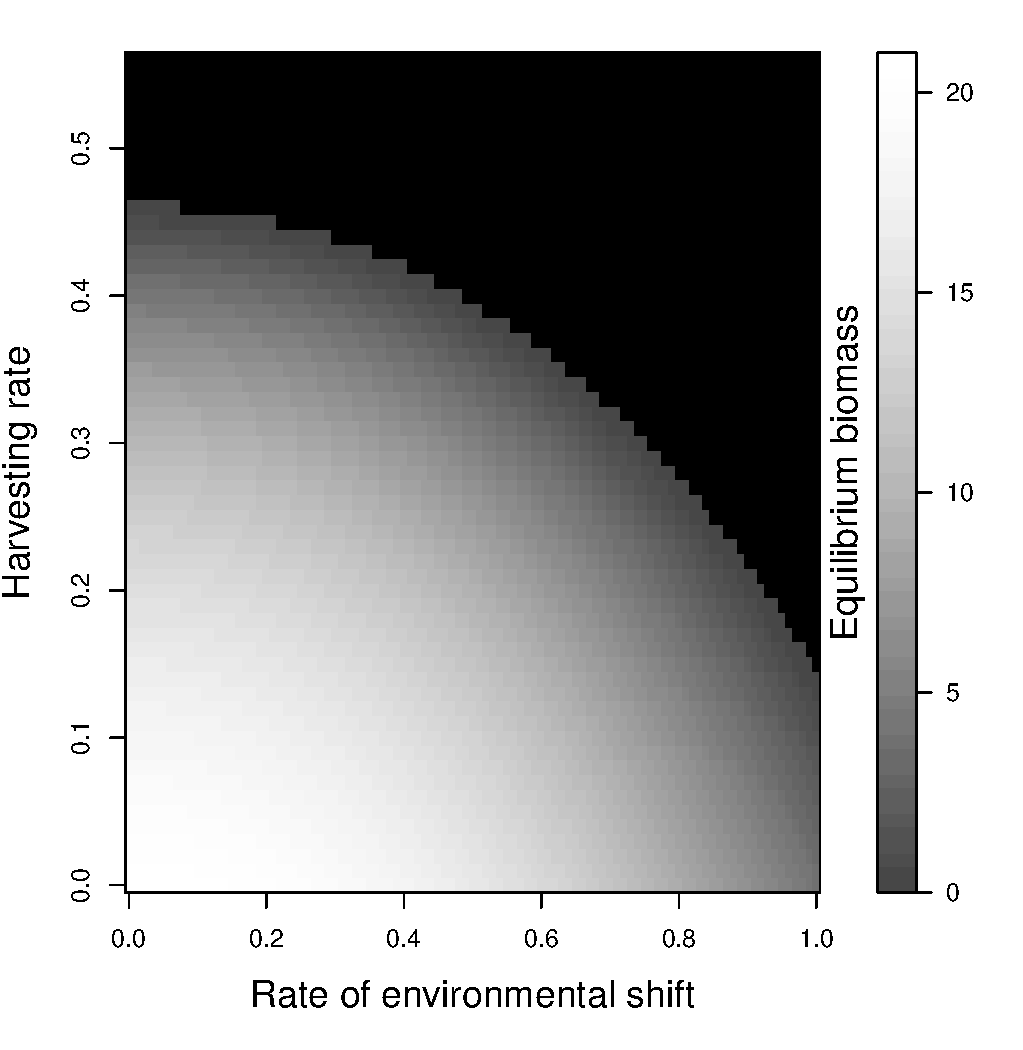
\includegraphics[width=\textwidth]{plots/eqbiomass.pdf}
\end{subfigure}
\begin{subfigure}{3in}
\subcaption{\label{rates}}
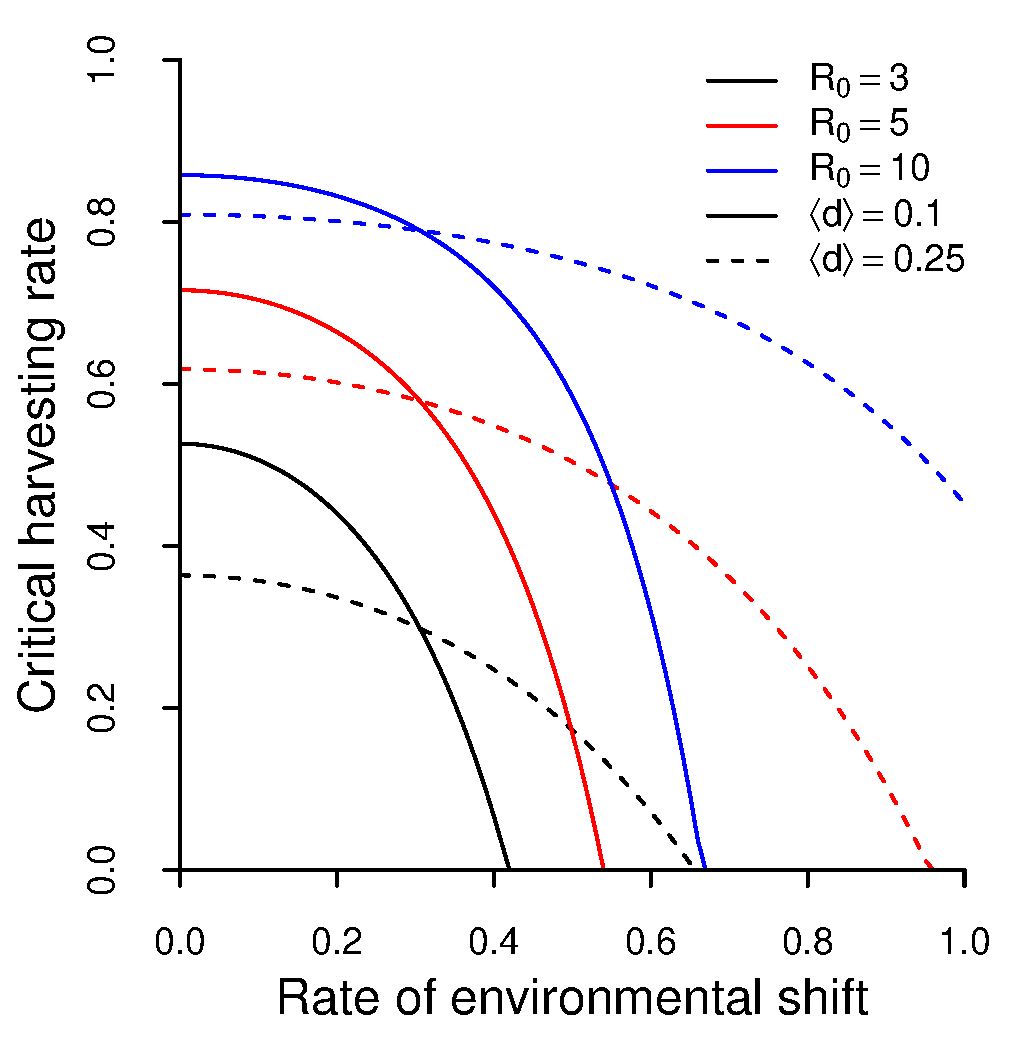
\includegraphics[width=\textwidth]{plots/critical_rates.pdf}
\end{subfigure}
\caption{(a) The equilibrium biomass of the population as a function of the rate of environmental shift on the x-axis and the harvesting rate on the y-axis. These results are from a Gaussian dispersal kernel with parameters $L=1$, $R_0=5$, $\langle d \rangle = 0.399$.  (b) The critical harvesting rate on the y-axis as a function of the rate of environmental shift on the x-axis.  Black lines correspond to a growth rate of $R_0=3$, red to $R_0=7$, and blue to $R_0=10$.  Solid lines correspond to an average dispersal distance $\langle d \rangle =0.1$ and dashed lines correspond to an average dispersal distance $\langle d \rangle =0.25$.  These results are from an approximated Gaussian dispersal kernel with $L=1$.}
\label{baseline}
\end{figure}

It is always the case that increasing the intrinsic growth rate, $R_0$, of the population increases the critical 
speed $c^*$ and the critical harvesting rate $h^*$, since a population that grows more quickly can recover 
more quickly from losses caused by these disturbances. However, whether or not dispersing farther is better 
depends on how quickly the environment is shifting (Figure \ref{baseline}). When the environment is shifting 
slowly, dispersing farther is detrimental since many larvae will disperse too far away from the viable patch. 
When the environment is shifting quickly, on the other hand, dispersing farther can help the population persist 
because some larvae will disperse into the space that will become viable shortly in the future.  This affects the critical harvesting rate: at a low rate of environmental shift, populations that disperse less can be harvested more severely than those that disperse further, whereas at a high rate of environmental shift, populations that disperse further can be harvested more severely.

We found positive synergy between the two stressors in our analysis of the Gaussian kernel (Figure \ref
{Synergy}).  In other words, a doubly stressed population loses more biomass than would be predicted from either stressor individually.  The stressors interact most strongly when they are both high, shortly before they drive the population extinct.  Our simulations with a Laplace kernel produce similar 
results. In the Appendix, we show analogous results for a sinusoidal dispersal kernel. 

\begin{figure}[htbp]
\begin{center}
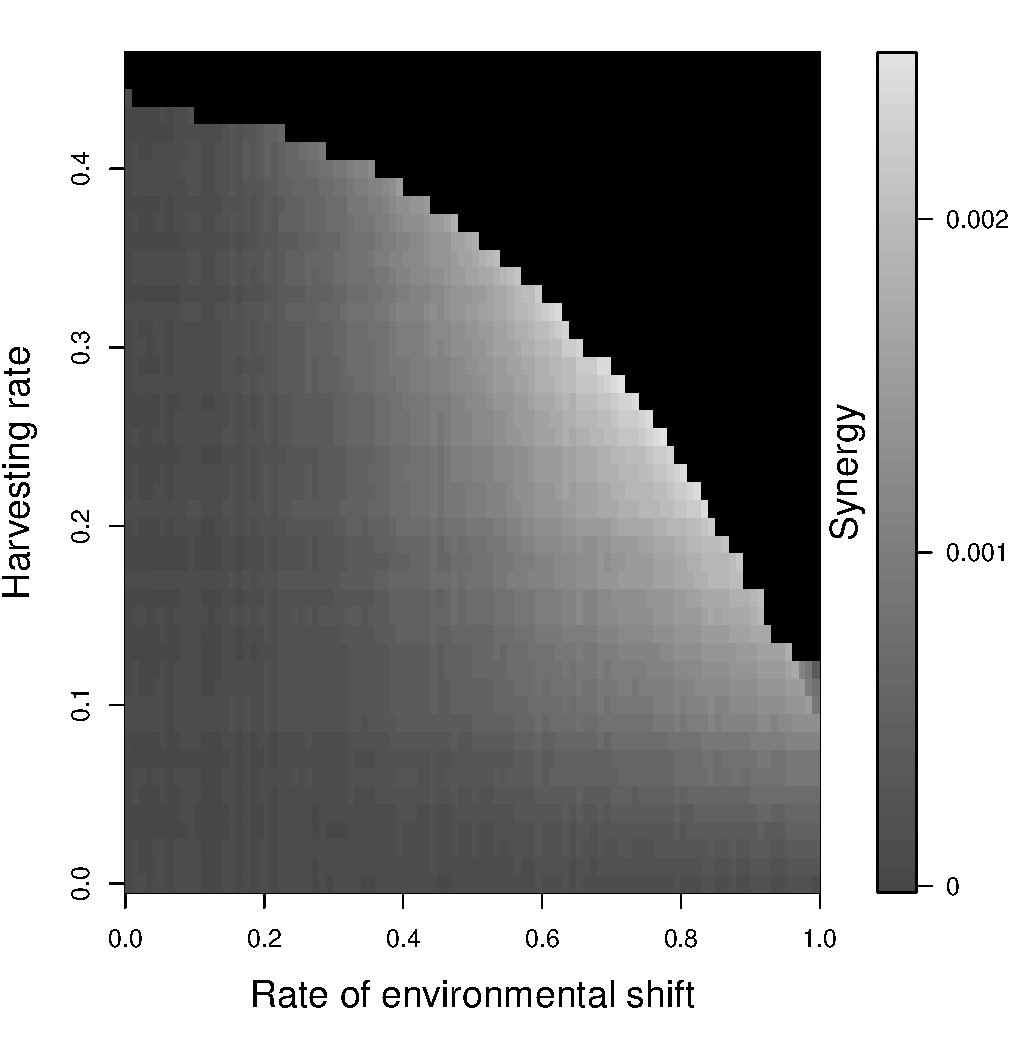
\includegraphics[width=3in]{plots/synergy.pdf}
\caption{Positive synergy between the two stressors.  The x-axis shows the rate of environmental shift, the y-axis shows the harvesting rate, and the color indicates the loss in biomass in the doubly stressed population in excess of the sum of the losses caused by each stressor individually, $E_\text{hc}-E_\text{h}-E_\text{c}$.  These results are from an approximated Gaussian dispersal kernel with parameters $L=1$, $R_0=5$, $\langle d \rangle = 0.399$.}
\label{Synergy}
\end{center}
\end{figure}

\subsection{Management Strategies }

We found that thresholds of any amount alleviate the effects of harvesting, and the ability of the population to 
persist is recovered (Figure \ref{thresholds}). Thus when thresholds are in place, the harvesting rate no longer 
determines the critical rate of environmental shift $c^*$. We also examined the effect of marine protected 
areas (MPAs) on the population's persistence to see whether it might extend the range of harvesting and 
climate change parameters where the fish population could survive. With MPAs in place, the population had a 
slightly higher abundance along the edges of the patch where the population is limited by harvesting, which 
translated into a slightly increased critical harvest rate (Figure \ref{MPAs}). Additionally MPAs increased 
overall catch at the highest harvest rates under which the population could survive (Figure \ref{MPAs}).

\begin{figure}[htbp]

\begin{subfigure}{.33\textwidth}
\subcaption{}
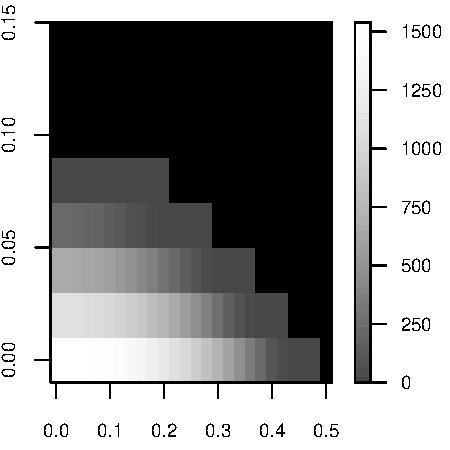
\includegraphics[width=\textwidth]{plots/eqbiomass_sim.pdf}
\end{subfigure}
\begin{subfigure}{.33\textwidth}
\subcaption{}
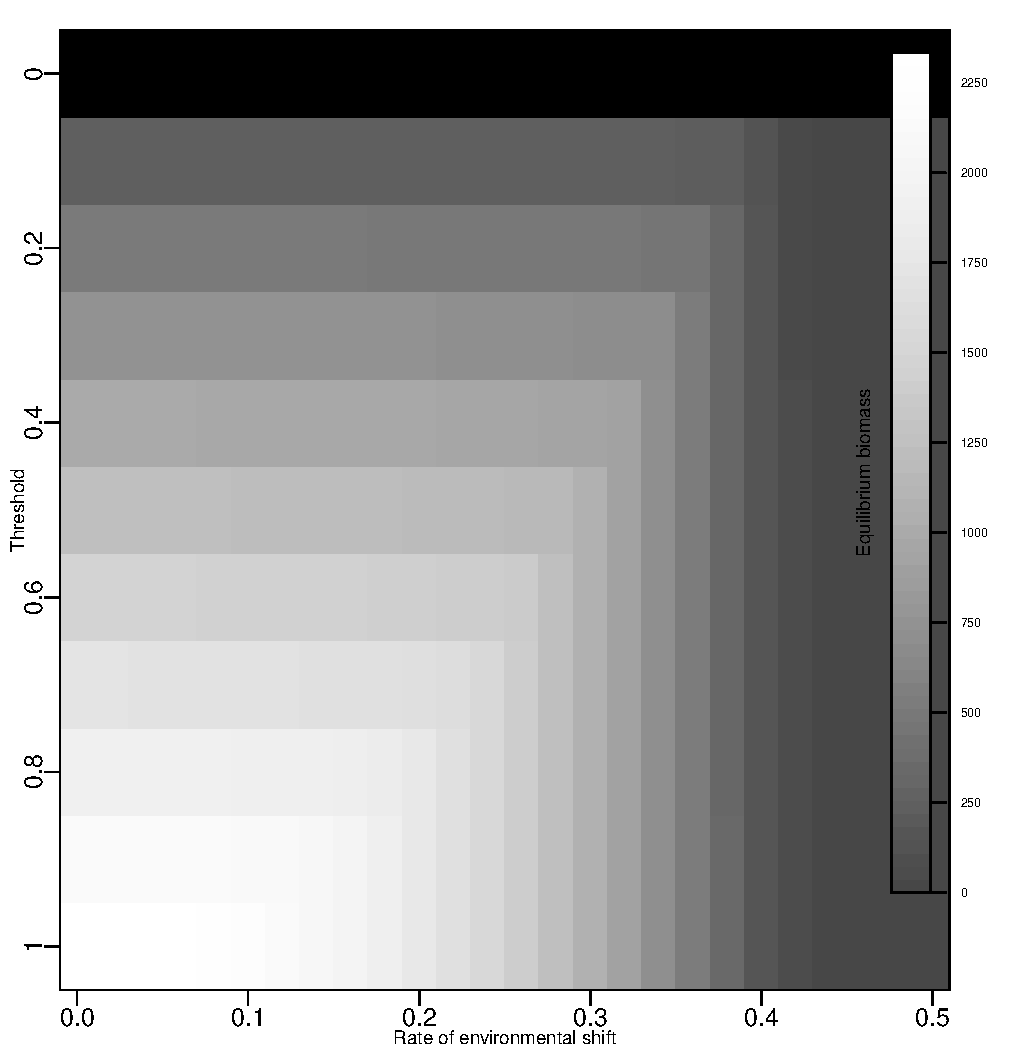
\includegraphics[width=\textwidth]{plots/eqbiomass_thresh.pdf}
\end{subfigure}
\begin{subfigure}{.33\textwidth}
\subcaption{}
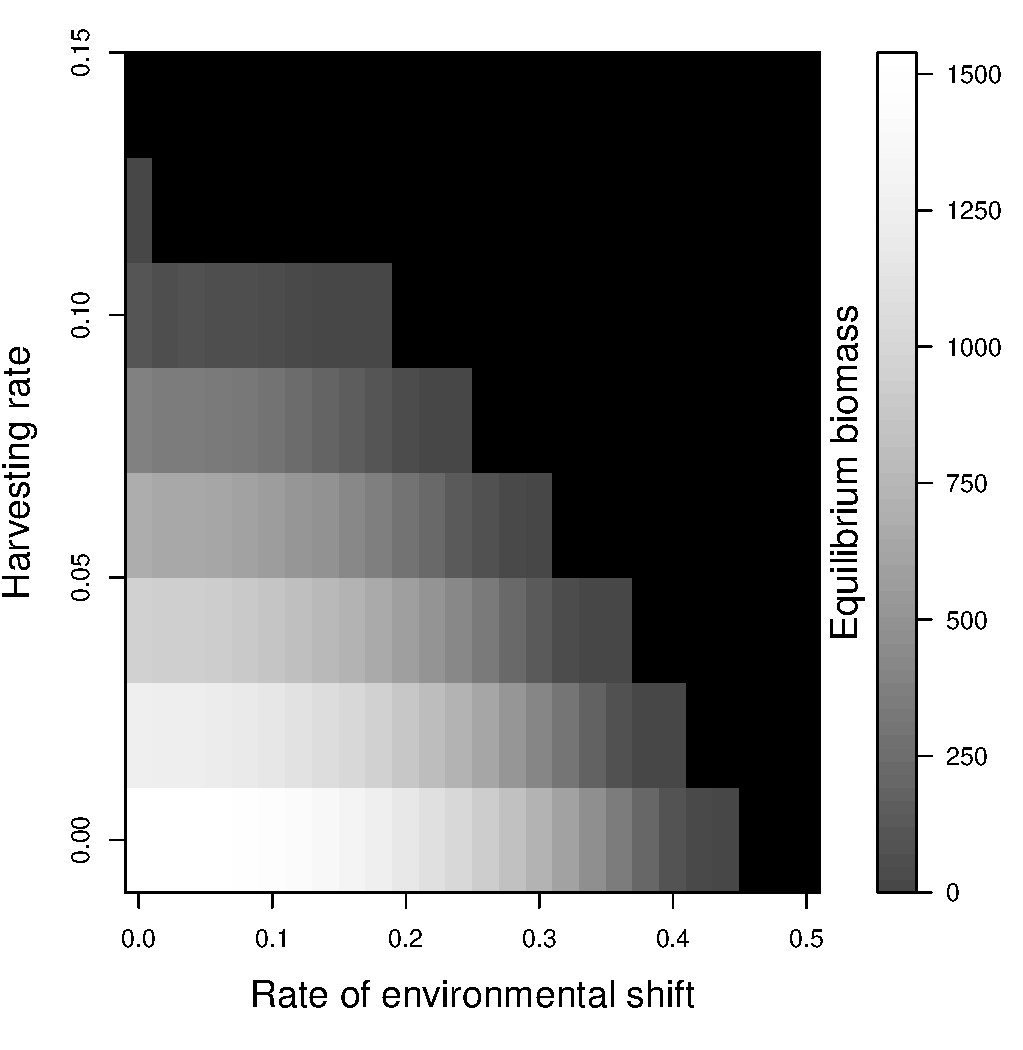
\includegraphics[width=\textwidth]{plots/eqbiomass_mpa.pdf}
\end{subfigure}
\caption{The equilibrium biomass of the population as a function of the rate of environmental shift on the x-axis and the harvesting rate on the y-axis with and without management strategies.  (a) No management.  (b) Threshold harvesting levels.  (c) MPAs.  These results are from a simulation with a Laplacian dispersal kernel with parameters $L=1$, $R_0=5$, $K=100$, and $\langle d \rangle =2$. }
\label{thresholds}
\end{figure}


\section{Discussion}

We extended the model of Zhou and Kot \citep{ZhouKot2011} to study a fish population subject to both the climate-driven range shifts already included and harvesting. Previous work has highlighted the importance of 
reproduction and dispersal to the vulnerability of fish populations to climate change \citep[\citet{Fordhametal2013}]
{Hastingsetal2005} and the integrodifference model explicitly includes these processes. We found that 
the two disturbances interact synergistically with each other in some cases. However, we also found that 
placing thresholds on harvesting intensity can alleviate interactions between the two stressors and that spatial 
management increased the maximum harvesting rate at which the population could survive.

We found that the synergy between the two stressors is positive and that the synergy is greatest in the region 
of parameter space where the equilibrium biomass is smallest. Additionally, we found that the higher the 
growth rate and the better the mean dispersal distance matches the rate of environmental shift, the better a 
population can adjust to harvest and climate change. We find similar results from the analytically derived 
biomass and the simulation derived biomass. This indicates that this result is robust to changes in the 
dispersal kernel. Similarly, in experiments, \cite{Moraetal2007} found no interaction between harvesting and 
habitat fragmentation but did find an interaction between harvesting and warming temperature \citep
{Moraetal2007}. We chose to measure the effect of each stressor by the drop in biomass caused by the 
stressor, as in \cite{Crainetal2008}. In general, measuring synergy additively is more conservative than 
measuring synergy multiplicatively: stressors that have positive multiplicative synergy may have zero additive 
synergy \citep{Crainetal2008, Foltetal1999}. Since we found small levels of positive additive synergy between 
the two stressors, other measures of synergy might show even higher levels of interaction. This synergy and 
the fact that it most severely affects those populations whose persistence is most tenuous is worrisome from a 
conservation perspective. Harvesting levels or rate of environment shift that are sustainable individually 
together can drive a population to extinction. It is therefore important to take the effects of both stressors into 
consideration when designing conservation and management strategies.

The two management strategies we modeled -- harvesting thresholds and MPAs -- both increased the 
population's biomass at equilibrium and improved its ability to persist. These management strategies also 
affect how the two stressors interact with each other.  Protected areas have 
been advanced as a way to help organisms keep pace with range shifts as well as to ameliorate anthropogenic disturbances like harvesting and habitat fragmentation\citep{Lawleretal2010, 
Hannahetal2007,Botsfordetal2001, Gaylordetal2005, 
HastingsBotsford2003,Thomasetal2012}.  While MPAs only change harvesting practices 
and do not directly address affect climate change, understanding how they ameliorate synergistic affects between harvesting 
and range shifts will help to better implement and place protected areas.

The advantage of a simple model like ours is that it is general enough to be applied to a number of systems.  However, it  ignores many of the complexities present in marine fisheries. We do 
not include Allee effects, so that even if the population shrank to very low levels it was possible for it to persist 
over time. However, we found that qualitatively similar results about the interaction between climate and 
harvesting would hold for a model with a recruitment function with Allee effect. We also did not include age 
structure in our model. The effects of both harvesting and climate change may be different across different age 
classes; including this level of complexity is left for future work. Additionally, we did not include any 
mechanisms aside from larval dispersal by which the population could keep up with a shifting climate.

In addition to these species-specific extensions, this modeling framework can easily be adjusted to consider 
species interactions, especially predator-prey pairs. Predatory species affect marine populations and 
considering a set of species that included both predators and prey would be equivalent to imposing additional 
stressors on the prey species whose interactions we would like to measure \citep{Lingetal2009, 
Gurevitchetal2000}. Considering multiple species would not only allow us to understand the effects of multiple 
stressors on prey populations but would also afford us the opportunity to study how community composition 
would change as a result of climate change, as has been observed in some marine systems \citep
{Urbanetal2012}.

Finally, our results suggest that particular combinations of harvesting and rate of environmental shift will affect 
some species more than others. Indeed, \citet{Perryetal2005} found that fish that shifted in response to 
warming in North Sea had faster life histories than non shifting species (smaller body sizes, faster maturation, 
smaller sizes at maturity). Using a simple mechanistic model like the one we presented can incorporate these 
species interactions and multiple disturbances to understand whether specific life histories are likely to be 
selected over others as harvesting and/or range shifts increase.

\bibliography{fish}
\section{Appendix}

As in Zhou et al. \citep{ZhouKot2011}, let $k(x-y)$ be a dispersal kernel and let $f(y)$ be a recruitment function.  The integrodifference model describing the population over time is given by 
\begin{equation} n_{t+1}(x)=\int_{-L/2+ct}^{L/2+ct}k(x-y)f(n_t(y))dy. \label{integro} \end{equation}

To find a traveling pulse, we are only interested in the population density as a function of the location within the patch rather than absolute position, $\overline{x}\equiv x-ct$.

\begin{equation}n^*(\overline{x})\equiv n^*(x-ct)=n_t(x).   \label{trav} \end{equation}

Then (\ref{integro}) giveas s us an expression for $n^*$:

\begin{align*}
n^*(\overline{x}-c)&=\int_{-L/2}^{L/2}k(\overline{x}-\overline{y})f(n^*(\overline{y}))d\overline y 
\\ \Rightarrow n^*(\overline{x})&=\int_{-L/2}^{L/2}k(\overline{x}+c-\overline{y})f(n^*(\overline{y}))d\overline y \tag{*} \label{pulse}
\end{align*}
If $f(0)=0$, $n^*(\overline{x})\equiv 0$ for all $\overline{x}\in[-L/2,L/2]$ is a trivial solution to this problem, i.e. if there are no fish anywhere there won't be at any time in the future. The population can be said to be persistent if the trivial traveling pulse is unstable since even when there are very small population levels, the population won't crash to $0$.  To evaluate stability (i.e. persistence), we will introduce a small perturbation to the traveling pulse $n^*(\overline{x})$,

\begin{align*}
n_t(x)&=n^*(\overline{x})+\xi_t(x)
\\ \Rightarrow \xi_{t+1}(x)&=\int_{-L/2+ct}^{L/2+ct}k(x-y)f'(n^*(\overline{y}))\xi_t(y)dy \text{ by linearizing around the traveling pulse and using (\ref{pulse})}
\\ \Rightarrow \xi_{t+1}(x)&=\int_{-L/2+ct}^{L/2+ct}k(x-y)f'(0)\xi_t(y)dy \text{ if we're interested in the stability of the trivial traveling pulse}
\end{align*}
If we assume $\xi_t(x)=\lambda^tu(x-ct)$ for some $\lambda\in\R$ and $u:[-L/2,L/2]\to\R$, then 
\begin{align*}
\lambda u(x-ct-c)&=f'(0)\int_{-L/2+ct}^{L/2+ct}k(x-y)u(y-ct)dy
\\ \lambda u(\overline{x})&=f'(0)\int_{-L/2}^{L/2}k(\overline{x}+c-\overline{y})u(\overline{y})dy
\end{align*}

Define the integral operator
$$ \psi_f(g)(x)=\int_{-L/2}^{L/2}f'(0)k(x+c-y)g(y)dy. $$
so that the perturbation to the traveling pulse will satisfy 
\begin{equation} \psi_f(u)(x)=\lambda u(x) \label{eigen} \end{equation}
Then the trivial traveling pulse is unstable when the dominant eigenvalue of $\psi_f$ is greater than $1$.

Let $f$ denote the recruitment function, let $h$ denote a harvesting function and let $m(y)=f(y-h(y))$, i.e. $m$ denotes the number of offspring after the adults have been harvested.  Note that $m'(0)=f'(0)(1-h'(0))$, assuming $h(0)=0$ (which must be the case).

Suppose $u$ is an eigenfunction of $\psi_f$ with eigenvalue $\lambda$.  Then 
\begin{align*}
\psi_m(u)(x)&=\int_{-L/2}^{L/2}m'(0)k(x+c-y)u(y)dy
\\&=(1-h'(0))\int_{-L/2}^{L/2}f'(0)k(x+c-y)u(y)dy
\\&=(1-h'(0))\psi_f(u)(x)
\\&=(1-h'(0))\lambda u(x)
\end{align*}
so that $u$ is also an eigenfuction of $\psi_m$, now with eigenvalue $(1-h'(0))\lambda$.

\subsection{Separable dispersal kernels }
Jentzsch's theorem shows that there is an eigenfunction $u$, provided that the kernel $k$ satisfy some properties.  Finding the eigenfunction is in general a hard problem to solve.  It becomes easier if the kernel $k$ is separable, i.e. there are functions $a_n,b_n$ such that $k(x-y)=\sum_{n=1}^\infty a_n(x)b_n(y)$.  In that case, (\ref{eigen}) becomes
\begin{align*}
\lambda u(x)&=f'(0)\sum_{n=1}^\infty\left( a_n(x)\int_{-L/2}^{L/2}b_n(y-c)u(y)dy\right)
\\ \Rightarrow \lambda\int_{-L/2}^{L/2}b_k(x-c)u(x)dx&=f'(0)\sum_{n=1}^{\infty}\left(\int_{-L/2}^{L/2}b_n(x-c)u(x)dx\right)\left(\int_{-L/2}^{L/2}a_n(y)b_k(y-c)dy\right)
\\ \Rightarrow \lambda d_k&=f'(0)\sum_{n=1}^\infty A_{nk}d_n  \tag{**} \label{problem}
\end{align*}
where
\begin{equation*}
A_{nk}=\int_{-L/2}^{L/2}a_n(x)b_k(x-c)dx \text{ and } d_k=\int_{-L/2}^{L/2}b_k(x-c)u(x)dx
\end{equation*}

\subsection{Gaussian dispersal kernel }
The Gaussian dispersal kernel is given by
$$k(|x-y|)=\frac{1}{2\sqrt{D\pi}}e^{\frac{-(x-y)^2}{4D}}.$$
As in \citep{Latore:1998fk}, this separable kernel can be written as
$$k(|x-y|)=\sum_{n=0}^\infty a_n(x)b_n(y)$$
where
$$a_n(x)=b_n(x)=\frac{1}{\sqrt{2n!\sqrt{D\pi}}}e^{-x^2/4D}\left(\frac{x}{\sqrt{2D}}\right)^n.$$

As a first approximation to $k$ we ignore all but the $0^{th}$ terms for $a_n$ and $b_n$ so that Equation \ref{problem} becomes
\begin{align*}
\lambda d_0(c)&=f'(0)A_{00}(c)d_0(c)
\\ \Rightarrow \lambda&=R_0(1-h)A_{00}(c)
\\\text{ where } A_{00}(c)&=2\sqrt{2}\exp\left(\frac{-c^2}{8D}\right)\left[\text{erf}\left(\frac{L-c}{2\sqrt{2D}}\right)-\text{erf}\left(\frac{-L-c}{2\sqrt{2D}}\right)\right]
\end{align*}
where $\text{erf}$ is the error function.  The critical rate of environmental shift $c^*$ and the critical harvesting rate $h^*$ are those values of $c$ and $h$, respectively, that make $\lambda=1$.

\subsection{Sinusoidal dispersal kernel }
A sinusoidal dispersal kernel is given by 
$$k(x-y)=\left\{\begin{array}{ccccc}
\frac{w}{2}\cos(w(x-y)) & , & |x-y|\leq\frac{\pi}{2w}
\\ 0 & , & |x-y|>\frac{\pi}{2w}
\end{array}\right.
$$
where $L$ is the length of the patch and we assume $\frac{\pi}{2w}>L,c<\frac{\pi}{2w}-L$.

In this case, $k(x-y)=\frac{w}{2}\cos(wx)\cos(w(y-c))+\frac{w}{2}\sin(wx)\sin(w(y-c))$ so that $A_{ij}$ and $d_i$ can be found for $i,j=1,2$ and (\ref{problem}) reduces to 
$$\lambda^2-\left(\frac{R_0(1-h)wL}{2}\cos(wc)\right)\lambda+\frac{R_0^2(1-h)^2}{16}\left(w^2L^2-\sin^2(wL)\right)=0.$$

If we solve for $\lambda$,we find
\begin{equation} \lambda=R_0(1-h)\left[\frac{wL\cos(wc)}{4}+\frac{1}{4}\sqrt{\sin^2(wL)-w^2L^2\sin^2(wc)}\right]. \label{cosine} \end{equation}


Zhou et al. \citep{ZhouKot2011} solve for the critical speed, $c^*$, at the population will be driven extinct:
$$c^*=c^*(R_0)=\frac{1}{w}\cos^{-1}\left[\frac{16+R_0^2(1-h)^2(w^2L^2-\sin^2(wL))}{8R_0(1-h)wL}\right].$$
Similarly, we can solve for the critical harvesting rate, $h^*$, at which the population will be driven extinct:
$$
h^*=1-\frac{1}{R_0}\cdot\frac{4wL}{w^2L^2-\sin^2(wL)}\left[\cos(wc)-\sqrt{\cos^2(wc)-1+\frac{\sin^2(wL)}{w^2L^2}}\right] 
$$

\subsection{Approximate Critical Harvesting Proportions}
~\\We will use the following Taylor series to make approximations of the critical harvesting proportions under the two dispersal kernels:
\begin{align*}
\cos(x)&=1-\frac{x^2}{2}
\\ \cos^2(x)&=1-x^2
\\ \sin^2(x)&=x^2-\frac{x^4}{3}
\\ erf(x)&=\frac{2}{\sqrt{\pi}}(x-\frac{x^3}{3})
\\ \exp(x)&=1+x+\frac{x^2}{2}
\end{align*}
For the sinusoidal kernel we found 
\begin{equation}
h^*=1-\frac{1}{R_0}\cdot\frac{4wL}{w^2L^2-\sin^2(wL)}\left[\cos(wc)-\sqrt{\cos^2(wc)-1+\frac{\sin^2(wL)}{w^2L^2}}\right] 
\end{equation} 
Using the Taylor series and the fact that $w=\frac{\sqrt{\frac{\pi^2}{4}-2}}{\sigma}$ where $\sigma^2$ is the variance of the sinusoidal kernel,
\begin{align*}
h^*&\sim 1-\frac{1}{R_0}\cdot\frac{12wL}{w^4L^4}\left[1-\frac{w^2c^2}{2}-\sqrt{1-w^2c^2-\frac{w^2L^2}{3}}\right]
%\\&=1-\frac{1}{R_0}\cdot\frac{12}{w^3L^3}\left[1-\frac{w^2c^2}{2}-\sqrt{1-w^2c^2-\frac{w^2L^2}{3}}\right]
%\\&=1-\frac{1}{R_0}\cdot\frac{12\sigma^3}{L^3(\frac{\pi^2}{4}-2)^{3/2}}\left[1-\frac{(\frac{\pi^2}{4}-2)c^2}{2\sigma^2}-\sqrt{1-\frac{(\frac{\pi^2}{4}-2)c^2}{\sigma^2}-\frac{(\frac{\pi^2}{4}-2)L^2}{3\sigma^2}}\right]
%\\&=1-\frac{1}{R_0}\cdot\frac{6\sigma}{L^3(\frac{\pi^2}{4}-2)^{3/2}}\left[2\sigma^2-(\frac{\pi^2}{4}-2)c^2-\frac{2}{\sqrt{3}}\sigma\sqrt{3\sigma^2-(\frac{\pi^2}{4}-2)3c^2-(\frac{\pi^2}{4}-2)L^2}\right]
%\\&=1-\frac{1}{R_0}\cdot\frac{6\sigma}{L^34(\frac{\pi^2}{4}-2)^{3/2}}\left[8\sigma^2-(\pi^2-8)c^2-\frac{4}{\sqrt{3}}\sigma\sqrt{12\sigma^2-(\pi^2-8)3c^2-(\pi^2-8)L^2}\right]
%\\&=1-\frac{12}{R_0L^3(\pi^2-8)^{3/2}}\cdot\sigma\left[8\sigma^2-(\pi^2-8)c^2-\frac{4}{\sqrt{3}}\sigma\sqrt{12\sigma^2-(\pi^2-8)3c^2-(\pi^2-8)L^2}\right]
\\&=1-\frac{1}{R_0}\cdot\frac{4\sqrt{3}}{L^3(\pi^2-8)^{3/2}}\cdot\sigma\left[8\sqrt{3}\sigma^2-(\pi^2-8)\sqrt{3}c^2-4\sigma\sqrt{12\sigma^2-(\pi^2-8)(3c^2+L^2)}\right]
\end{align*}
For the Gaussian kernel we found 
\begin{equation}
h^*=1-\frac{2\sqrt{2}\exp\left(\frac{c^{2}}{8D}\right)}{R_0\left[erf\left(\frac{L-c}{2\sqrt{2D}}\right)-erf\left(\frac{-L-c}{2\sqrt{2D}}\right)\right]}
\end{equation} 
Using the Taylor series and the fact that $D=\frac{\sigma^2}{2}$ where $\sigma^2$ is the variance of the exponential kernel,
\begin{align*}
h^*&\sim 1-\frac{\sqrt{2\pi}(1+\frac{c^2}{8D}+\frac{c^4}{128D^2})}{R_0\sqrt{\pi}\left[\frac{L-c}{2\sqrt{2D}}-\frac{(L-c)^3}{3(2\sqrt{2D})^3}-\frac{-L-c}{2\sqrt{2D}}+\frac{(-L-c)^3}{3(2\sqrt{2D})^3)}\right]}
%\\&= 1-\frac{\sqrt{2\pi}(1+\frac{c^2}{8D}+\frac{c^4}{128D^2})}{R_0\left[\frac{2L}{2\sqrt{2D}}+\frac{-L^3+3L^2c-3Lc^2+c^3-L^3-3L^2c-3Lc^2-c^3}{3(2\sqrt{2D})^3}\right]}
%\\&= 1-\frac{\sqrt{2\pi}(1+\frac{c^2}{8D}+\frac{c^4}{128D^2})}{R_0\left[\frac{L}{\sqrt{2D}}-2\frac{L^3+3Lc^2}{3(2\sqrt{2D})^3}\right]}
%\\&= 1-\frac{\sqrt{2\pi}(1+\frac{c^2}{8D}+\frac{c^4}{128D^2})}{R_0L\left[\frac{48D-2(L^2+3c^2)}{3(2\sqrt{2D})^3}\right]}
%\\&= 1-\frac{3*32D\sqrt{D\pi}(1+\frac{c^2}{8D}+\frac{c^4}{128D^2})}{R_0L\left(48D-2(L^2+3c^2)\right)}
%\\&= 1-\frac{3*32D\sqrt{D\pi}(\frac{128D^2+16c^2D+c^4}{128D^2})}{R_0L\left(48D-2(L^2+3c^2)\right)}
%\\&= 1-\frac{3\sqrt{\pi}(128D^2+16c^2D+c^4)}{4R_0L\sqrt{D}\left(48D-2(L^2+3c^2)\right)}
%\\&= 1-\frac{3\sqrt{2\pi}(32\sigma^4+8c^2\sigma^2+c^4)}{4R_0L\sigma\left(24\sigma^2-2(L^2+3c^2)\right)}
\\&= 1-\frac{1}{R_0}\cdot\frac{3\sqrt{2\pi}}{8L}\frac{(32\sigma^4+8c^2\sigma^2+c^4)}{\sigma\left(12\sigma^2-(L^2+3c^2)\right)}
\end{align*}
In the case of both kernels, the critical harvesting proportion can be approximated by a function that looks like 
\begin{equation}
h^*\sim1- \frac{1}{R_0}\cdot C(L)f(\sigma^2,c^2,L^2+3c^2)
\end{equation}
where $C(L,R_0)$ is a decreasing function of the length of the viable patch and the intrinsic growth rate.


\end{document}
